% ==================================================================
% APPENDIX A3 — Cosmic Chronometers: extraction of ε.
%
% FINAL DRAFT on freeze-checkpoint numbers (2026-04-19).
% Numerics: scripts/epsilon_convergence/ch4_cosmic_chronometers.py
% Background: scripts/epsilon_convergence/ect_background.py
%
% Structure (unified per-probe template shared with A1, A2, A4-A5):
%   A3.1  Physics of the probe
%   A3.2  Observational inputs
%   A3.3  ECT-side model and extraction scope
%   A3.4  Extraction statistic
%   A3.5  Interval definition and origin of the width
%   A3.6  Figure
%   A3.7  Methodological limitations
%
% Character of this channel (GPT r21):
%   Direct late-time expansion probe; one-sided upper bound under
%   physical prior; true consistency channel, not primary extraction.
%
% NO integration into preprint yet.
% ==================================================================

\section{Extraction of the effective uniform-$\varepsilon$ interval
from the cosmic chronometers channel}
\label{app:eps_extraction_cc}

This appendix derives the effective uniform-$\varepsilon$ interval
from the cosmic chronometers channel used in the rebuilt \S15.5.
Unlike the Hubble + $r_s$ channel of A1, which uses a shift in the
CMB-inferred $H_0$ together with a sound-horizon anchor, the
cosmic chronometers channel directly constrains the late-time
Hubble rate $H(z)$ at $0 \lesssim z \lesssim 2$ through the
differential ageing of passively evolving stellar populations. As
a result, it is a direct probe of late-time expansion history and
does not require any matter-era or recombination-era modelling. In
the present retained-pipeline it functions as a late-time
consistency channel: it admits a broad one-sided upper bound on
$\varepsilon$ after imposing the physical prior
$\varepsilon \geq 0$, and does not by itself extract a non-trivial
lower edge in the physical region.

\subsection*{A3.1\quad Physics of the probe}

The cosmic chronometers technique measures the Hubble rate at
cosmological redshifts by treating the differential ageing of
massive, passively evolving galaxies as an effective clock:
\begin{equation}
H(z) \;=\; -\frac{1}{1+z}\,\frac{dz}{dt},
\end{equation}
where $dz/dt$ is estimated from pairs of such galaxies at close
but distinct redshifts, so that $dt$ is inferred from stellar
population synthesis. The method requires no cosmological
distance-ladder, no sound-horizon anchor, and no high-redshift
extrapolation; its systematics are dominated by stellar-population
modelling rather than by cosmological assumptions. In the
effective uniform-$\varepsilon$ layer of
\S\ref{subsec:eps_def_rebuilt}, the $\varepsilon$-deformation enters
the late-time Hubble rate directly through
\eqref{eq:eps_friedmann_A1}, and the present channel tests whether
a non-zero $\varepsilon$ is compatible with this ensemble of
$H(z)$ measurements.

\subsection*{A3.2\quad Observational inputs}

The data used here is a representative subset of the Moresco+2022
cosmic chronometers compilation \cite{Moresco2022}, consisting of
31 measurements of $H(z)$ at $z \in [0.07,\,1.97]$. Each
measurement is treated as Gaussian with diagonal observational
uncertainty $\sigma_{H_i}$, ranging from approximately
$4~\mathrm{km\,s^{-1}\,Mpc^{-1}}$ at the most precise points to
$\sim 60~\mathrm{km\,s^{-1}\,Mpc^{-1}}$ at the least-constrained
ones. The full off-diagonal covariance of the Moresco+2022
compilation, which includes shared systematic contributions from
stellar population synthesis modelling, is not used at this
proxy level; the present treatment is therefore optimistic on
statistical weight and represents an upper bound on the
constraining power of the channel.

\subsection*{A3.3\quad ECT-side model and extraction scope}

Under the uniform-$\varepsilon$ ansatz, the model prediction at
each data redshift is computed through the common background
module (\texttt{ect\_background.py}) as
\begin{equation}
H_{\rm ECT}(z,\, H_0,\, \varepsilon)
\;=\; H_0 \cdot E_{\rm ECT}(z,\, \varepsilon),
\end{equation}
with $E_{\rm ECT}$ given by \eqref{eq:eps_friedmann_A1}. The fit
has two free parameters: $\varepsilon$ (the primary quantity of
interest) and $H_0$ (profiled over). Since the cosmic chronometers
data do not directly anchor the absolute normalisation of $H(z)$,
$H_0$ is profiled rather than fixed, which broadens the constraint
on $\varepsilon$ relative to any anchored analysis.

\paragraph{Held fixed under the present proxy.}
$\Omega_m = 0.315$, $\Omega_\Lambda$, $\Omega_r$; the diagonal
observational uncertainty structure (no off-diagonal covariance);
the Moresco+2022 compilation as external input.

\paragraph{Varied.}
Both $\varepsilon$ and $H_0$ are varied. $\varepsilon$ is scanned
over a one-dimensional grid; at each value of $\varepsilon$,
$H_0$ is optimised by bounded scalar minimisation over
$H_0 \in [50,\,100]~\mathrm{km\,s^{-1}\,Mpc^{-1}}$.

\paragraph{Not included at this proxy level.}
The full Moresco+2022 covariance with shared stellar-population
systematics; a joint fit of $(\Omega_m, H_0, \varepsilon)$ with
$\Omega_m$ floated; redshift-dependence of the
stellar-population-modelling systematic; late-time deviations from
the uniform-$\varepsilon$ ansatz.

\subsection*{A3.4\quad Extraction statistic}

The extraction statistic is the profile chi-squared
\begin{equation}
\chi^2(\varepsilon) \;=\;
\min_{H_0}\,\sum_{i=1}^{31}
\left[\,\frac{H_i^{\rm obs} - H_{\rm ECT}(z_i, H_0, \varepsilon)}
{\sigma_{H_i}}\,\right]^{\!2}.
\label{eq:chi2_cc_eps}
\end{equation}
The best-fit is defined by the minimum of $\chi^2(\varepsilon)$,
the $1\sigma$ interval by $\Delta\chi^2 \leq 1$, and the $2\sigma$
interval by $\Delta\chi^2 \leq 4$, computed directly on the
one-dimensional profile.

\subsection*{A3.5\quad Interval definition and origin of the width}

\paragraph{Numerical outcome.}
Direct numerical evaluation through the common background module
yields
\begin{align}
\varepsilon_*
&\;=\; +0.005,
\\[2pt]
H_0^{\rm prof}(\varepsilon_*)
&\;\approx\; 68.2~\mathrm{km\,s^{-1}\,Mpc^{-1}},
\\[2pt]
\chi^2_{\min} / {\rm dof}
&\;\approx\; 14.5 / 29.
\end{align}
The raw $1\sigma$ interval (before imposing any physical prior)
covers $\varepsilon \in [-0.020,\,+0.087]$; the raw $2\sigma$
interval extends from $-0.020$ to the scan upper edge
$+0.150$. The best-fit $\varepsilon_*$ is statistically
indistinguishable from zero, and the profile is very shallow:
within $\Delta\chi^2 \leq 1$ the data admits any value of
$\varepsilon$ in a broad range surrounding zero.

\paragraph{Imposing the physical prior.}
Under the physical prior $\varepsilon \geq 0$ of
\S\ref{subsec:eps_def_rebuilt}, the cosmic chronometers channel
admits
\begin{equation}
[\varepsilon_{\rm lo}^{1\sigma},\,\varepsilon_{\rm hi}^{1\sigma}]
\;=\;
[\,0,\ 0.087\,],
\qquad
[\varepsilon_{\rm lo}^{2\sigma},\,\varepsilon_{\rm hi}^{2\sigma}]
\;=\;
[\,0,\ 0.150\,].
\label{eq:eps_cc_retained}
\end{equation}
The lower edges are set by the physical prior rather than by the
data, and the channel functions as a one-sided upper bound in the
physical region.

\paragraph{Origin of the width.}
The $1\sigma$ upper edge $\approx 0.087$ reflects the curvature of
$\chi^2(\varepsilon)$ at fixed profiled $H_0$ under the assumed
diagonal observational uncertainty structure. The dominant
contribution to this width is the statistical uncertainty of the
individual $H(z)$ measurements; the profiling of $H_0$ absorbs
any overall normalisation shift, so the extracted
$\varepsilon$-constraint is driven purely by the redshift-dependent
\emph{shape} of $H(z)$. The constraint is weak because
$E_{\rm ECT}(z, \varepsilon)$ is only mildly sensitive to
$\varepsilon$ in the data redshift range $z < 2$: the
$(1+z)^{2\varepsilon}$ factor enters multiplicatively but is close
to unity at small $\varepsilon$ and moderate $z$, so the
data lever-arm is modest.

\paragraph{Channel character.}
In the language of
\S\ref{subsec:eps_retained_rebuilt}, the cosmic chronometers
channel is a consistency channel rather than a primary extraction
channel. Its principal role in the retained-five-probe intersection
is to exclude large values of $\varepsilon$ at late times
--- in particular, to limit the uniform-$\varepsilon$ ansatz to
values compatible with the observed $H(z)$ shape in
$z < 2$. It does not contribute a lower edge to the joint band; the
binding lower edge of the retained interval is set by the JWST
channel of A2.

\subsection*{A3.6\quad Figure}

\begin{figure}[H]
\centering
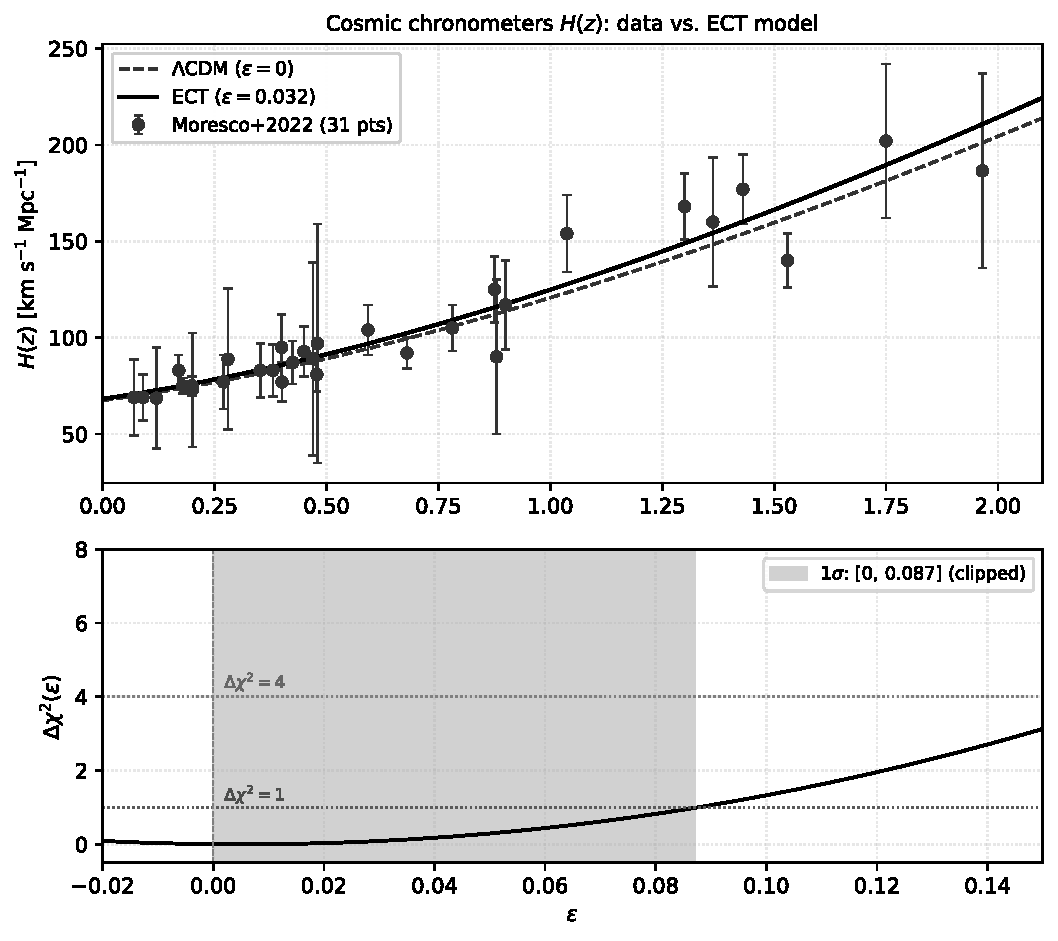
\includegraphics[width=0.82\textwidth]{figures/fig_cc_extraction_bw.pdf}
\caption{Extraction of the effective $\varepsilon$-interval from
the cosmic chronometers channel, under the common background
module of Appendix~\ref{app:eps_methodology}. Top panel: data
points of Moresco+2022 (31 measurements, $z \in [0.07,\,1.97]$)
shown with error bars; the $\Lambda$CDM best-fit curve (dotted)
and the ECT curve at the retained-band central value
$\varepsilon = 0.032$ (solid) are overlaid. Bottom panel: profile
$\chi^2(\varepsilon)$ with $\Delta\chi^2 = 1$ and $\Delta\chi^2 = 4$
levels marked as horizontal gray lines; the raw minimum near
$\varepsilon \approx +0.005$ is indistinguishable from zero within
the data. All shading and line styles are grayscale per preprint
convention.}
\label{fig:cc_extraction}
\end{figure}

\subsection*{A3.7\quad Methodological limitations}

\textit{(i) Diagonal covariance only.}
The full Moresco+2022 covariance has substantial off-diagonal
contributions from shared stellar-population systematics. Their
inclusion would broaden the $1\sigma$ and $2\sigma$ intervals
modestly; the present treatment is therefore more optimistic than
a fully correlated analysis.

\textit{(ii) $\Omega_m$ held fixed.}
Cosmic chronometers cannot simultaneously determine $\Omega_m$,
$H_0$, and $\varepsilon$ without external priors. Fixing
$\Omega_m = 0.315$ at the $\Lambda$CDM-best-fit value, as in the
common background module, is a standard proxy choice; letting
$\Omega_m$ float broadens the constraint on $\varepsilon$
considerably and reduces the channel to a near-trivial constraint.

\textit{(iii) $\Lambda$CDM-background common proxy.}
As in A1.7(i) and A2.8(ii), the common background module uses a
$\Lambda$CDM-best-fit parameter set as external input; the
$\varepsilon$-deformation is applied on top. A closure-level
background would replace this proxy.

\textit{(iv) Sub-compilation of Moresco+2022.}
The present analysis uses a representative 31-point subset of the
published Moresco+2022 compilation rather than the full catalogue.
The extracted upper bound is representative but not maximally
constraining.

% ==================================================================
% END Appendix (extraction, cosmic chronometers channel).
% ==================================================================
